% J. Mieses - J. R. Capablanca, Berlin, 1913, with Capablanca's notes.
% Build with: python3 ../../tools/chessbook.py game-08-mieses-capablanca.tex
\documentclass[10pt,twoside]{article}
\usepackage[paperwidth=487.56bp,paperheight=691.65bp,top=72pt,bottom=44pt,inner=50pt,outer=48pt,
            headheight=13pt,headsep=20pt,footskip=0pt]{geometry}
\usepackage[T1]{fontenc}
\usepackage[lining]{ebgaramond}
\usepackage{graphicx}
\usepackage{microtype}
\usepackage{tikz}
\usepackage{fancyhdr}
\usepackage[hidelinks,pdftitle={Mieses - Capablanca, Berlin, 1913},
            pdfauthor={J. R. Capablanca}]{hyperref}

\newcommand{\textsizebook}{\fontsize{10.5}{12.6}\selectfont}
\AtBeginDocument{\textsizebook}
\setlength{\columnsep}{11pt}
\setlength{\parindent}{9pt}
\setlength{\parskip}{0pt}
\setlength{\emergencystretch}{1.5em}
\raggedbottom

\newlength{\boardwidth}
\setlength{\boardwidth}{160pt}

% A main line move, as a bold heading above its note
\newcommand{\Move}[1]{\par\addvspace{8pt}\noindent\phantomsection{\bfseries #1}\par\nopagebreak}
% A diagram in the text
\newcommand{\ChessDiagram}[1]{\par\addvspace{7pt}{\centering #1\par}\addvspace{5pt}}

\pagestyle{fancy}
\fancyhf{}
\renewcommand{\headrulewidth}{0pt}
\fancyhead[LE,RO]{\thepage}
\fancyhead[CE]{Centre Game}
\fancyhead[CO]{Mieses -- Capablanca}







\newcommand{\figK}{\raisebox{-0.14em}{
\includegraphics[height=1em]{diagrams/figK}}}
\newcommand{\figQ}{\raisebox{-0.14em}{
\includegraphics[height=1em]{diagrams/figQ}}}
\newcommand{\figR}{\raisebox{-0.14em}{
\includegraphics[height=1em]{diagrams/figR}}}
\newcommand{\figB}{\raisebox{-0.14em}{
\includegraphics[height=1em]{diagrams/figB}}}
\newcommand{\figN}{\raisebox{-0.14em}{
\includegraphics[height=1em]{diagrams/figN}}}
\begin{document}

\twocolumn[{%
\thispagestyle{empty}
\begin{tikzpicture}[remember picture,overlay]
  \node[circle,draw=black,line width=1.6pt,fill=black!20,minimum size=112pt] (seal)
       at ([xshift=75pt,yshift=-75pt]current page.north west) {};
  \draw[line width=0.9pt] ([shift={(-48pt,-30pt)}]seal.center) -- ([shift={(44pt,34pt)}]seal.center);
  \node[rotate=37] at ([shift={(-11pt,14pt)}]seal.center) {\fontsize{25}{25}\selectfont\bfseries Game};
  \node[rotate=37] at ([shift={(10pt,-16pt)}]seal.center) {\fontsize{38}{38}\selectfont\bfseries 8};
  \node[anchor=north east] at ([xshift=-14pt,yshift=-24pt]current page.north east)
       {\href{https://lichess.org/analysis/pgn/e4_e5_d4_exd4_Qxd4_Nc6_Qe3_Nf6}{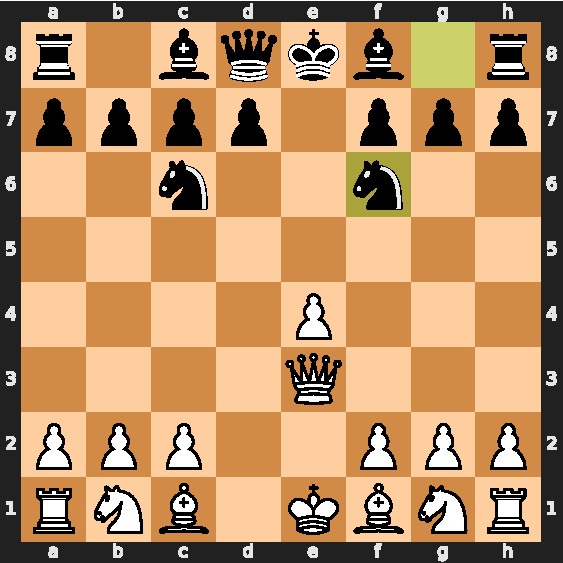
\includegraphics[width=108pt]{diagrams/board-374aac3ba7f6}}};
\end{tikzpicture}

\vspace*{38pt}
\begin{center}
  \begin{minipage}{235pt}\centering
    {\fontsize{22}{25}\selectfont\bfseries Centre Game\par}
    \vspace{4pt}\rule{\linewidth}{1pt}\\[-9.5pt]\rule{\linewidth}{0.4pt}
  \end{minipage}

  \vspace{14pt}
  {\fontsize{19}{22}\selectfont\bfseries Mieses -- Capablanca\par}
  \vspace{10pt}
  {\fontsize{15}{18}\selectfont\bfseries Berlin, 1913\par}
  \vspace{8pt}
  {\fontsize{11}{13}\selectfont White: J. Mieses \quad Black: J. R. Capablanca\par}
  \vspace{10pt}
  {\centering\fontsize{8.5}{10}\selectfont\itshape
   Notes by J. R. Capablanca, from \textup{Chess Fundamentals} (1921), which is in the public domain.\\
   Descriptive notation has been converted to algebraic. Page references are to the book.\\
   Click any move or diagram to open it on Lichess.\par}
\end{center}
\vspace{10pt}
}]
\textsizebook

\Move{\href{https://lichess.org/analysis/pgn/e4}{1.e4} \href{https://lichess.org/analysis/pgn/e4_e5}{e5} \href{https://lichess.org/analysis/pgn/e4_e5_d4}{2.d4} \href{https://lichess.org/analysis/pgn/e4_e5_d4_exd4}{exd4} \href{https://lichess.org/analysis/pgn/e4_e5_d4_exd4_Qxd4}{3.\figQ xd4} \href{https://lichess.org/analysis/pgn/e4_e5_d4_exd4_Qxd4_Nc6}{\figN c6} \href{https://lichess.org/analysis/pgn/e4_e5_d4_exd4_Qxd4_Nc6_Qe3}{4.\figQ e3} \href{https://lichess.org/analysis/pgn/e4_e5_d4_exd4_Qxd4_Nc6_Qe3_Nf6}{\figN f6} \href{https://lichess.org/analysis/pgn/e4_e5_d4_exd4_Qxd4_Nc6_Qe3_Nf6_Nc3}{5.\figN c3} \href{https://lichess.org/analysis/pgn/e4_e5_d4_exd4_Qxd4_Nc6_Qe3_Nf6_Nc3_Bb4}{\figB b4} \href{https://lichess.org/analysis/pgn/e4_e5_d4_exd4_Qxd4_Nc6_Qe3_Nf6_Nc3_Bb4_Bd2}{6.\figB d2} \href{https://lichess.org/analysis/pgn/e4_e5_d4_exd4_Qxd4_Nc6_Qe3_Nf6_Nc3_Bb4_Bd2_O-O}{0--0} \href{https://lichess.org/analysis/pgn/e4_e5_d4_exd4_Qxd4_Nc6_Qe3_Nf6_Nc3_Bb4_Bd2_O-O_O-O-O}{7.0--0--0} \href{https://lichess.org/analysis/pgn/e4_e5_d4_exd4_Qxd4_Nc6_Qe3_Nf6_Nc3_Bb4_Bd2_O-O_O-O-O_Re8}{\figR e8}}

In this position, instead of the text move, \href{https://lichess.org/analysis/pgn/e4_e5_d4_exd4_Qxd4_Nc6_Qe3_Nf6_Nc3_Bb4_Bd2_O-O_O-O-O_d6}{7...d6} is often played in order to develop the Queen's Bishop. My idea was to exert sufficient pressure against the e-pawn to win it, and thus gain a material advantage, which would, at least, compensate whatever slight advantage of position White might have. The plan, I think, is quite feasible, my subsequent difficulties being due to faulty execution of the plan.

\Move{\href{https://lichess.org/analysis/pgn/e4_e5_d4_exd4_Qxd4_Nc6_Qe3_Nf6_Nc3_Bb4_Bd2_O-O_O-O-O_Re8_Qg3}{8.\figQ g3} \href{https://lichess.org/analysis/pgn/e4_e5_d4_exd4_Qxd4_Nc6_Qe3_Nf6_Nc3_Bb4_Bd2_O-O_O-O-O_Re8_Qg3_Nxe4}{\figN xe4} \href{https://lichess.org/analysis/pgn/e4_e5_d4_exd4_Qxd4_Nc6_Qe3_Nf6_Nc3_Bb4_Bd2_O-O_O-O-O_Re8_Qg3_Nxe4_Nxe4}{9.\figN xe4} \href{https://lichess.org/analysis/pgn/e4_e5_d4_exd4_Qxd4_Nc6_Qe3_Nf6_Nc3_Bb4_Bd2_O-O_O-O-O_Re8_Qg3_Nxe4_Nxe4_Rxe4}{\figR xe4} \href{https://lichess.org/analysis/pgn/e4_e5_d4_exd4_Qxd4_Nc6_Qe3_Nf6_Nc3_Bb4_Bd2_O-O_O-O-O_Re8_Qg3_Nxe4_Nxe4_Rxe4_Bf4}{10.\figB f4}}

\ChessDiagram{\href{https://lichess.org/analysis/pgn/e4_e5_d4_exd4_Qxd4_Nc6_Qe3_Nf6_Nc3_Bb4_Bd2_O-O_O-O-O_Re8_Qg3_Nxe4_Nxe4_Rxe4_Bf4}{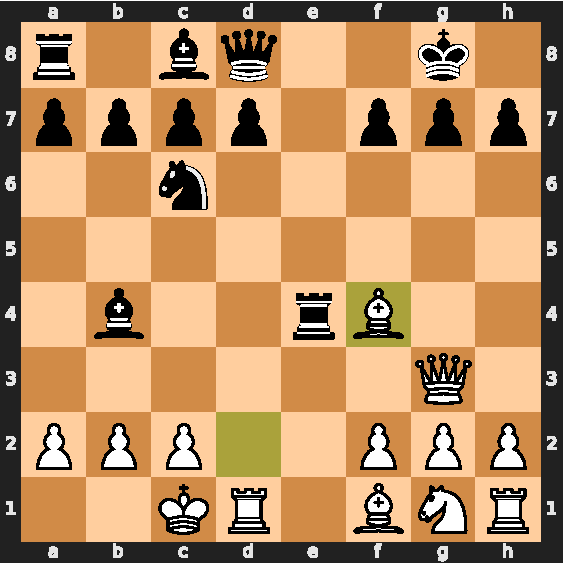
\includegraphics[width=\boardwidth]{diagrams/board-9f9a3062aac0}}}

\Move{\href{https://lichess.org/analysis/pgn/e4_e5_d4_exd4_Qxd4_Nc6_Qe3_Nf6_Nc3_Bb4_Bd2_O-O_O-O-O_Re8_Qg3_Nxe4_Nxe4_Rxe4_Bf4_Qf6}{10...\figQ f6}}

White's threat to regain the Pawn was merely with the idea of gaining time to develop his pieces. Black could have played \href{https://lichess.org/analysis/pgn/e4_e5_d4_exd4_Qxd4_Nc6_Qe3_Nf6_Nc3_Bb4_Bd2_O-O_O-O-O_Re8_Qg3_Nxe4_Nxe4_Rxe4_Bf4_d6}{10...d6}; opening the way for his Queen's Bishop, when would have followed, \href{https://lichess.org/analysis/pgn/e4_e5_d4_exd4_Qxd4_Nc6_Qe3_Nf6_Nc3_Bb4_Bd2_O-O_O-O-O_Re8_Qg3_Nxe4_Nxe4_Rxe4_Bf4_d6_Bd3}{11.\figB d3} \href{https://lichess.org/analysis/pgn/e4_e5_d4_exd4_Qxd4_Nc6_Qe3_Nf6_Nc3_Bb4_Bd2_O-O_O-O-O_Re8_Qg3_Nxe4_Nxe4_Rxe4_Bf4_d6_Bd3_Re8}{\figR e8} \href{https://lichess.org/analysis/pgn/e4_e5_d4_exd4_Qxd4_Nc6_Qe3_Nf6_Nc3_Bb4_Bd2_O-O_O-O-O_Re8_Qg3_Nxe4_Nxe4_Rxe4_Bf4_d6_Bd3_Re8_Nf3}{12.\figN f3}, and White would soon start a powerful direct attack against Black's King. With the text move Black aims at taking the initiative away from White in accordance with the principles laid down in this book.

\Move{\href{https://lichess.org/analysis/pgn/e4_e5_d4_exd4_Qxd4_Nc6_Qe3_Nf6_Nc3_Bb4_Bd2_O-O_O-O-O_Re8_Qg3_Nxe4_Nxe4_Rxe4_Bf4_Qf6_Nh3}{11.\figN h3}}

If \href{https://lichess.org/analysis/pgn/e4_e5_d4_exd4_Qxd4_Nc6_Qe3_Nf6_Nc3_Bb4_Bd2_O-O_O-O-O_Re8_Qg3_Nxe4_Nxe4_Rxe4_Bf4_Qf6_Bxc7}{11.\figB xc7} \href{https://lichess.org/analysis/pgn/e4_e5_d4_exd4_Qxd4_Nc6_Qe3_Nf6_Nc3_Bb4_Bd2_O-O_O-O-O_Re8_Qg3_Nxe4_Nxe4_Rxe4_Bf4_Qf6_Bxc7_d6}{d6}; and White's Bishop would be completely shut off, and could only be extricated, if at all, with serious loss of position. The text move aims at quick development to keep the initiative.

\Move{\href{https://lichess.org/analysis/pgn/e4_e5_d4_exd4_Qxd4_Nc6_Qe3_Nf6_Nc3_Bb4_Bd2_O-O_O-O-O_Re8_Qg3_Nxe4_Nxe4_Rxe4_Bf4_Qf6_Nh3_d6}{11...d6}}

This now is not only a developing move, but it also threatens to win a piece by \figB xh3.

\Move{\href{https://lichess.org/analysis/pgn/e4_e5_d4_exd4_Qxd4_Nc6_Qe3_Nf6_Nc3_Bb4_Bd2_O-O_O-O-O_Re8_Qg3_Nxe4_Nxe4_Rxe4_Bf4_Qf6_Nh3_d6_Bd3}{12.\figB d3} \href{https://lichess.org/analysis/pgn/e4_e5_d4_exd4_Qxd4_Nc6_Qe3_Nf6_Nc3_Bb4_Bd2_O-O_O-O-O_Re8_Qg3_Nxe4_Nxe4_Rxe4_Bf4_Qf6_Nh3_d6_Bd3_Nd4}{\figN d4}}

This complicates the game unnecessarily. \href{https://lichess.org/analysis/pgn/e4_e5_d4_exd4_Qxd4_Nc6_Qe3_Nf6_Nc3_Bb4_Bd2_O-O_O-O-O_Re8_Qg3_Nxe4_Nxe4_Rxe4_Bf4_Qf6_Nh3_d6_Bd3_Re8}{12...\figR e8}; was simple, and perfectly safe.

\Move{\href{https://lichess.org/analysis/pgn/e4_e5_d4_exd4_Qxd4_Nc6_Qe3_Nf6_Nc3_Bb4_Bd2_O-O_O-O-O_Re8_Qg3_Nxe4_Nxe4_Rxe4_Bf4_Qf6_Nh3_d6_Bd3_Nd4_Be3}{13.\figB e3}}

\ChessDiagram{\href{https://lichess.org/analysis/pgn/e4_e5_d4_exd4_Qxd4_Nc6_Qe3_Nf6_Nc3_Bb4_Bd2_O-O_O-O-O_Re8_Qg3_Nxe4_Nxe4_Rxe4_Bf4_Qf6_Nh3_d6_Bd3_Nd4_Be3}{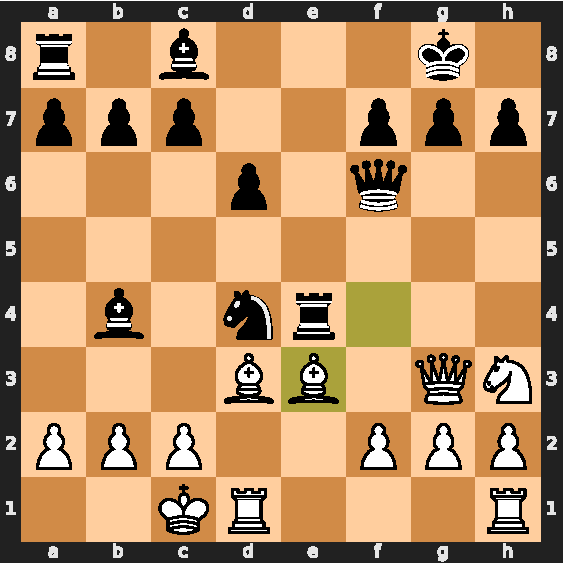
\includegraphics[width=\boardwidth]{diagrams/board-0eea446162c9}}}

\Move{\href{https://lichess.org/analysis/pgn/e4_e5_d4_exd4_Qxd4_Nc6_Qe3_Nf6_Nc3_Bb4_Bd2_O-O_O-O-O_Re8_Qg3_Nxe4_Nxe4_Rxe4_Bf4_Qf6_Nh3_d6_Bd3_Nd4_Be3_Bg4}{13...\figB g4}}

This is a serious mistake. The position was most interesting, and though in appearance dangerous for Black, not so in reality. The right move would have been \href{https://lichess.org/analysis/pgn/e4_e5_d4_exd4_Qxd4_Nc6_Qe3_Nf6_Nc3_Bb4_Bd2_O-O_O-O-O_Re8_Qg3_Nxe4_Nxe4_Rxe4_Bf4_Qf6_Nh3_d6_Bd3_Nd4_Be3_Rg4}{13...\figR g4}, when we would have \href{https://lichess.org/analysis/pgn/e4_e5_d4_exd4_Qxd4_Nc6_Qe3_Nf6_Nc3_Bb4_Bd2_O-O_O-O-O_Re8_Qg3_Nxe4_Nxe4_Rxe4_Bf4_Qf6_Nh3_d6_Bd3_Nd4_Be3_Rg4_Bxd4}{14.\figB xd4} \href{https://lichess.org/analysis/pgn/e4_e5_d4_exd4_Qxd4_Nc6_Qe3_Nf6_Nc3_Bb4_Bd2_O-O_O-O-O_Re8_Qg3_Nxe4_Nxe4_Rxe4_Bf4_Qf6_Nh3_d6_Bd3_Nd4_Be3_Rg4_Bxd4_Rxd4}{\figR xd4} \href{https://lichess.org/analysis/pgn/e4_e5_d4_exd4_Qxd4_Nc6_Qe3_Nf6_Nc3_Bb4_Bd2_O-O_O-O-O_Re8_Qg3_Nxe4_Nxe4_Rxe4_Bf4_Qf6_Nh3_d6_Bd3_Nd4_Be3_Rg4_Bxd4_Rxd4_c3}{15.c3} \href{https://lichess.org/analysis/pgn/e4_e5_d4_exd4_Qxd4_Nc6_Qe3_Nf6_Nc3_Bb4_Bd2_O-O_O-O-O_Re8_Qg3_Nxe4_Nxe4_Rxe4_Bf4_Qf6_Nh3_d6_Bd3_Nd4_Be3_Rg4_Bxd4_Rxd4_c3_Bxc3}{\figB xc3} \href{https://lichess.org/analysis/pgn/e4_e5_d4_exd4_Qxd4_Nc6_Qe3_Nf6_Nc3_Bb4_Bd2_O-O_O-O-O_Re8_Qg3_Nxe4_Nxe4_Rxe4_Bf4_Qf6_Nh3_d6_Bd3_Nd4_Be3_Rg4_Bxd4_Rxd4_c3_Bxc3_bxc3}{16.bxc3} \href{https://lichess.org/analysis/pgn/e4_e5_d4_exd4_Qxd4_Nc6_Qe3_Nf6_Nc3_Bb4_Bd2_O-O_O-O-O_Re8_Qg3_Nxe4_Nxe4_Rxe4_Bf4_Qf6_Nh3_d6_Bd3_Nd4_Be3_Rg4_Bxd4_Rxd4_c3_Bxc3_bxc3_Rg4}{\figR g4} \href{https://lichess.org/analysis/pgn/e4_e5_d4_exd4_Qxd4_Nc6_Qe3_Nf6_Nc3_Bb4_Bd2_O-O_O-O-O_Re8_Qg3_Nxe4_Nxe4_Rxe4_Bf4_Qf6_Nh3_d6_Bd3_Nd4_Be3_Rg4_Bxd4_Rxd4_c3_Bxc3_bxc3_Rg4_Qe3}{17.\figQ e3} (best), \href{https://lichess.org/analysis/pgn/e4_e5_d4_exd4_Qxd4_Nc6_Qe3_Nf6_Nc3_Bb4_Bd2_O-O_O-O-O_Re8_Qg3_Nxe4_Nxe4_Rxe4_Bf4_Qf6_Nh3_d6_Bd3_Nd4_Be3_Rg4_Bxd4_Rxd4_c3_Bxc3_bxc3_Rg4_Qe3_Qxc3}{17...\figQ xc3+} \href{https://lichess.org/analysis/pgn/e4_e5_d4_exd4_Qxd4_Nc6_Qe3_Nf6_Nc3_Bb4_Bd2_O-O_O-O-O_Re8_Qg3_Nxe4_Nxe4_Rxe4_Bf4_Qf6_Nh3_d6_Bd3_Nd4_Be3_Rg4_Bxd4_Rxd4_c3_Bxc3_bxc3_Rg4_Qe3_Qxc3_Bc2}{18.\figB c2} \href{https://lichess.org/analysis/pgn/e4_e5_d4_exd4_Qxd4_Nc6_Qe3_Nf6_Nc3_Bb4_Bd2_O-O_O-O-O_Re8_Qg3_Nxe4_Nxe4_Rxe4_Bf4_Qf6_Nh3_d6_Bd3_Nd4_Be3_Rg4_Bxd4_Rxd4_c3_Bxc3_bxc3_Rg4_Qe3_Qxc3_Bc2_Qxe3}{\figQ xe3+} \href{https://lichess.org/analysis/pgn/e4_e5_d4_exd4_Qxd4_Nc6_Qe3_Nf6_Nc3_Bb4_Bd2_O-O_O-O-O_Re8_Qg3_Nxe4_Nxe4_Rxe4_Bf4_Qf6_Nh3_d6_Bd3_Nd4_Be3_Rg4_Bxd4_Rxd4_c3_Bxc3_bxc3_Rg4_Qe3_Qxc3_Bc2_Qxe3_fxe3}{19.fxe3} \href{https://lichess.org/analysis/pgn/e4_e5_d4_exd4_Qxd4_Nc6_Qe3_Nf6_Nc3_Bb4_Bd2_O-O_O-O-O_Re8_Qg3_Nxe4_Nxe4_Rxe4_Bf4_Qf6_Nh3_d6_Bd3_Nd4_Be3_Rg4_Bxd4_Rxd4_c3_Bxc3_bxc3_Rg4_Qe3_Qxc3_Bc2_Qxe3_fxe3_Rxg2}{\figR xg2}, and Black has the best of the game with four Pawns for a Knight, besides the fact that all the White Pawns are isolated.

\Move{\href{https://lichess.org/analysis/pgn/e4_e5_d4_exd4_Qxd4_Nc6_Qe3_Nf6_Nc3_Bb4_Bd2_O-O_O-O-O_Re8_Qg3_Nxe4_Nxe4_Rxe4_Bf4_Qf6_Nh3_d6_Bd3_Nd4_Be3_Bg4_Ng5}{14.\figN g5!} \href{https://lichess.org/analysis/pgn/e4_e5_d4_exd4_Qxd4_Nc6_Qe3_Nf6_Nc3_Bb4_Bd2_O-O_O-O-O_Re8_Qg3_Nxe4_Nxe4_Rxe4_Bf4_Qf6_Nh3_d6_Bd3_Nd4_Be3_Bg4_Ng5_Rxe3}{\figR xe3}}

There was nothing better.

\Move{\href{https://lichess.org/analysis/pgn/e4_e5_d4_exd4_Qxd4_Nc6_Qe3_Nf6_Nc3_Bb4_Bd2_O-O_O-O-O_Re8_Qg3_Nxe4_Nxe4_Rxe4_Bf4_Qf6_Nh3_d6_Bd3_Nd4_Be3_Bg4_Ng5_Rxe3_Qxg4}{15.\figQ xg4!} \href{https://lichess.org/analysis/pgn/e4_e5_d4_exd4_Qxd4_Nc6_Qe3_Nf6_Nc3_Bb4_Bd2_O-O_O-O-O_Re8_Qg3_Nxe4_Nxe4_Rxe4_Bf4_Qf6_Nh3_d6_Bd3_Nd4_Be3_Bg4_Ng5_Rxe3_Qxg4_Ne2}{\figN e2+}}

\ChessDiagram{\href{https://lichess.org/analysis/pgn/e4_e5_d4_exd4_Qxd4_Nc6_Qe3_Nf6_Nc3_Bb4_Bd2_O-O_O-O-O_Re8_Qg3_Nxe4_Nxe4_Rxe4_Bf4_Qf6_Nh3_d6_Bd3_Nd4_Be3_Bg4_Ng5_Rxe3_Qxg4_Ne2}{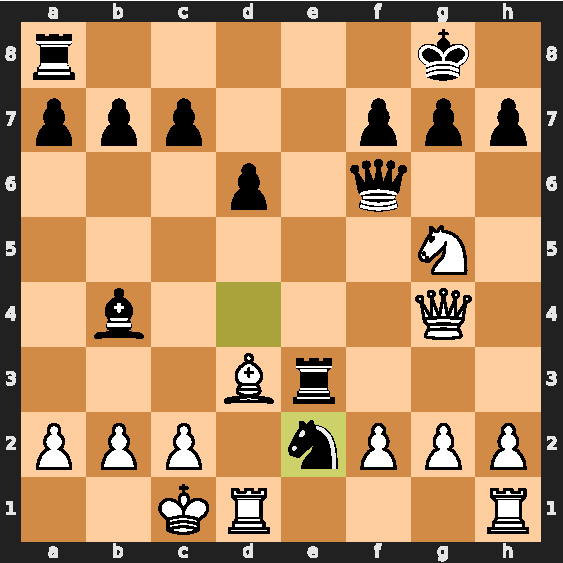
\includegraphics[width=\boardwidth]{diagrams/board-2935e8ef58b3}}}

\Move{\href{https://lichess.org/analysis/pgn/e4_e5_d4_exd4_Qxd4_Nc6_Qe3_Nf6_Nc3_Bb4_Bd2_O-O_O-O-O_Re8_Qg3_Nxe4_Nxe4_Rxe4_Bf4_Qf6_Nh3_d6_Bd3_Nd4_Be3_Bg4_Ng5_Rxe3_Qxg4_Ne2_Bxe2}{16.\figB xe2!} \href{https://lichess.org/analysis/pgn/e4_e5_d4_exd4_Qxd4_Nc6_Qe3_Nf6_Nc3_Bb4_Bd2_O-O_O-O-O_Re8_Qg3_Nxe4_Nxe4_Rxe4_Bf4_Qf6_Nh3_d6_Bd3_Nd4_Be3_Bg4_Ng5_Rxe3_Qxg4_Ne2_Bxe2_Rxe2}{\figR xe2} \href{https://lichess.org/analysis/pgn/e4_e5_d4_exd4_Qxd4_Nc6_Qe3_Nf6_Nc3_Bb4_Bd2_O-O_O-O-O_Re8_Qg3_Nxe4_Nxe4_Rxe4_Bf4_Qf6_Nh3_d6_Bd3_Nd4_Be3_Bg4_Ng5_Rxe3_Qxg4_Ne2_Bxe2_Rxe2_Ne4}{17.\figN e4!} \href{https://lichess.org/analysis/pgn/e4_e5_d4_exd4_Qxd4_Nc6_Qe3_Nf6_Nc3_Bb4_Bd2_O-O_O-O-O_Re8_Qg3_Nxe4_Nxe4_Rxe4_Bf4_Qf6_Nh3_d6_Bd3_Nd4_Be3_Bg4_Ng5_Rxe3_Qxg4_Ne2_Bxe2_Rxe2_Ne4_Rxe4}{\figR xe4} \href{https://lichess.org/analysis/pgn/e4_e5_d4_exd4_Qxd4_Nc6_Qe3_Nf6_Nc3_Bb4_Bd2_O-O_O-O-O_Re8_Qg3_Nxe4_Nxe4_Rxe4_Bf4_Qf6_Nh3_d6_Bd3_Nd4_Be3_Bg4_Ng5_Rxe3_Qxg4_Ne2_Bxe2_Rxe2_Ne4_Rxe4_Qxe4}{18.\figQ xe4} \href{https://lichess.org/analysis/pgn/e4_e5_d4_exd4_Qxd4_Nc6_Qe3_Nf6_Nc3_Bb4_Bd2_O-O_O-O-O_Re8_Qg3_Nxe4_Nxe4_Rxe4_Bf4_Qf6_Nh3_d6_Bd3_Nd4_Be3_Bg4_Ng5_Rxe3_Qxg4_Ne2_Bxe2_Rxe2_Ne4_Rxe4_Qxe4_Qg5}{\figQ g5+} \href{https://lichess.org/analysis/pgn/e4_e5_d4_exd4_Qxd4_Nc6_Qe3_Nf6_Nc3_Bb4_Bd2_O-O_O-O-O_Re8_Qg3_Nxe4_Nxe4_Rxe4_Bf4_Qf6_Nh3_d6_Bd3_Nd4_Be3_Bg4_Ng5_Rxe3_Qxg4_Ne2_Bxe2_Rxe2_Ne4_Rxe4_Qxe4_Qg5_f4}{19.f4} \href{https://lichess.org/analysis/pgn/e4_e5_d4_exd4_Qxd4_Nc6_Qe3_Nf6_Nc3_Bb4_Bd2_O-O_O-O-O_Re8_Qg3_Nxe4_Nxe4_Rxe4_Bf4_Qf6_Nh3_d6_Bd3_Nd4_Be3_Bg4_Ng5_Rxe3_Qxg4_Ne2_Bxe2_Rxe2_Ne4_Rxe4_Qxe4_Qg5_f4_Qb5}{\figQ b5} \href{https://lichess.org/analysis/pgn/e4_e5_d4_exd4_Qxd4_Nc6_Qe3_Nf6_Nc3_Bb4_Bd2_O-O_O-O-O_Re8_Qg3_Nxe4_Nxe4_Rxe4_Bf4_Qf6_Nh3_d6_Bd3_Nd4_Be3_Bg4_Ng5_Rxe3_Qxg4_Ne2_Bxe2_Rxe2_Ne4_Rxe4_Qxe4_Qg5_f4_Qb5_c3}{20.c3} \href{https://lichess.org/analysis/pgn/e4_e5_d4_exd4_Qxd4_Nc6_Qe3_Nf6_Nc3_Bb4_Bd2_O-O_O-O-O_Re8_Qg3_Nxe4_Nxe4_Rxe4_Bf4_Qf6_Nh3_d6_Bd3_Nd4_Be3_Bg4_Ng5_Rxe3_Qxg4_Ne2_Bxe2_Rxe2_Ne4_Rxe4_Qxe4_Qg5_f4_Qb5_c3_Bc5}{\figB c5} \href{https://lichess.org/analysis/pgn/e4_e5_d4_exd4_Qxd4_Nc6_Qe3_Nf6_Nc3_Bb4_Bd2_O-O_O-O-O_Re8_Qg3_Nxe4_Nxe4_Rxe4_Bf4_Qf6_Nh3_d6_Bd3_Nd4_Be3_Bg4_Ng5_Rxe3_Qxg4_Ne2_Bxe2_Rxe2_Ne4_Rxe4_Qxe4_Qg5_f4_Qb5_c3_Bc5_Rhe1}{21.\figR he1} \href{https://lichess.org/analysis/pgn/e4_e5_d4_exd4_Qxd4_Nc6_Qe3_Nf6_Nc3_Bb4_Bd2_O-O_O-O-O_Re8_Qg3_Nxe4_Nxe4_Rxe4_Bf4_Qf6_Nh3_d6_Bd3_Nd4_Be3_Bg4_Ng5_Rxe3_Qxg4_Ne2_Bxe2_Rxe2_Ne4_Rxe4_Qxe4_Qg5_f4_Qb5_c3_Bc5_Rhe1_Qc6}{\figQ c6} \href{https://lichess.org/analysis/pgn/e4_e5_d4_exd4_Qxd4_Nc6_Qe3_Nf6_Nc3_Bb4_Bd2_O-O_O-O-O_Re8_Qg3_Nxe4_Nxe4_Rxe4_Bf4_Qf6_Nh3_d6_Bd3_Nd4_Be3_Bg4_Ng5_Rxe3_Qxg4_Ne2_Bxe2_Rxe2_Ne4_Rxe4_Qxe4_Qg5_f4_Qb5_c3_Bc5_Rhe1_Qc6_Rd5}{22.\figR d5}}

\href{https://lichess.org/analysis/pgn/e4_e5_d4_exd4_Qxd4_Nc6_Qe3_Nf6_Nc3_Bb4_Bd2_O-O_O-O-O_Re8_Qg3_Nxe4_Nxe4_Rxe4_Bf4_Qf6_Nh3_d6_Bd3_Nd4_Be3_Bg4_Ng5_Rxe3_Qxg4_Ne2_Bxe2_Rxe2_Ne4_Rxe4_Qxe4_Qg5_f4_Qb5_c3_Bc5_Rhe1_Qc6_Qxc6}{22.\figQ xc6} would have given White a decided advantage, enough to win with proper play. Mieses, however, feared the difficulties of an ending where, while having the exchange, he would be a Pawn minus. He preferred to keep the Queens on the board and keep up the attack. At first sight, and even after careful thought, there seems to be no objection to his plan; but in truth such is not the case. From this point the game will gradually improve in Black's favour until, with the exchange ahead, White is lost.

\Move{\href{https://lichess.org/analysis/pgn/e4_e5_d4_exd4_Qxd4_Nc6_Qe3_Nf6_Nc3_Bb4_Bd2_O-O_O-O-O_Re8_Qg3_Nxe4_Nxe4_Rxe4_Bf4_Qf6_Nh3_d6_Bd3_Nd4_Be3_Bg4_Ng5_Rxe3_Qxg4_Ne2_Bxe2_Rxe2_Ne4_Rxe4_Qxe4_Qg5_f4_Qb5_c3_Bc5_Rhe1_Qc6_Rd5_Qd7}{22...\figQ d7} \href{https://lichess.org/analysis/pgn/e4_e5_d4_exd4_Qxd4_Nc6_Qe3_Nf6_Nc3_Bb4_Bd2_O-O_O-O-O_Re8_Qg3_Nxe4_Nxe4_Rxe4_Bf4_Qf6_Nh3_d6_Bd3_Nd4_Be3_Bg4_Ng5_Rxe3_Qxg4_Ne2_Bxe2_Rxe2_Ne4_Rxe4_Qxe4_Qg5_f4_Qb5_c3_Bc5_Rhe1_Qc6_Rd5_Qd7_f5}{23.f5} \href{https://lichess.org/analysis/pgn/e4_e5_d4_exd4_Qxd4_Nc6_Qe3_Nf6_Nc3_Bb4_Bd2_O-O_O-O-O_Re8_Qg3_Nxe4_Nxe4_Rxe4_Bf4_Qf6_Nh3_d6_Bd3_Nd4_Be3_Bg4_Ng5_Rxe3_Qxg4_Ne2_Bxe2_Rxe2_Ne4_Rxe4_Qxe4_Qg5_f4_Qb5_c3_Bc5_Rhe1_Qc6_Rd5_Qd7_f5_c6}{c6} \href{https://lichess.org/analysis/pgn/e4_e5_d4_exd4_Qxd4_Nc6_Qe3_Nf6_Nc3_Bb4_Bd2_O-O_O-O-O_Re8_Qg3_Nxe4_Nxe4_Rxe4_Bf4_Qf6_Nh3_d6_Bd3_Nd4_Be3_Bg4_Ng5_Rxe3_Qxg4_Ne2_Bxe2_Rxe2_Ne4_Rxe4_Qxe4_Qg5_f4_Qb5_c3_Bc5_Rhe1_Qc6_Rd5_Qd7_f5_c6_Rd2}{24.\figR d2} \href{https://lichess.org/analysis/pgn/e4_e5_d4_exd4_Qxd4_Nc6_Qe3_Nf6_Nc3_Bb4_Bd2_O-O_O-O-O_Re8_Qg3_Nxe4_Nxe4_Rxe4_Bf4_Qf6_Nh3_d6_Bd3_Nd4_Be3_Bg4_Ng5_Rxe3_Qxg4_Ne2_Bxe2_Rxe2_Ne4_Rxe4_Qxe4_Qg5_f4_Qb5_c3_Bc5_Rhe1_Qc6_Rd5_Qd7_f5_c6_Rd2_d5}{d5}}

\ChessDiagram{\href{https://lichess.org/analysis/pgn/e4_e5_d4_exd4_Qxd4_Nc6_Qe3_Nf6_Nc3_Bb4_Bd2_O-O_O-O-O_Re8_Qg3_Nxe4_Nxe4_Rxe4_Bf4_Qf6_Nh3_d6_Bd3_Nd4_Be3_Bg4_Ng5_Rxe3_Qxg4_Ne2_Bxe2_Rxe2_Ne4_Rxe4_Qxe4_Qg5_f4_Qb5_c3_Bc5_Rhe1_Qc6_Rd5_Qd7_f5_c6_Rd2_d5}{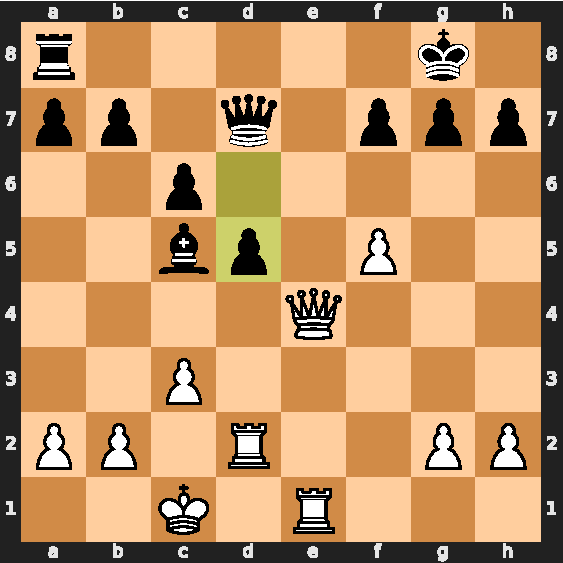
\includegraphics[width=\boardwidth]{diagrams/board-560ac589ba13}}}

My plan for the moment is very simple. It will consist in bringing my Bishop around to f6. Then I shall try to paralyse White's attack against my King by playing ...h6, and also prevent White from ever playing g5. Once my King is safe from attack I shall begin to advance my Queen's side Pawns, where there are four to three; and that advantage, coupled with the enormous attacking power of my Bishop at f6, will at least assure me an even chance of success.

\Move{\href{https://lichess.org/analysis/pgn/e4_e5_d4_exd4_Qxd4_Nc6_Qe3_Nf6_Nc3_Bb4_Bd2_O-O_O-O-O_Re8_Qg3_Nxe4_Nxe4_Rxe4_Bf4_Qf6_Nh3_d6_Bd3_Nd4_Be3_Bg4_Ng5_Rxe3_Qxg4_Ne2_Bxe2_Rxe2_Ne4_Rxe4_Qxe4_Qg5_f4_Qb5_c3_Bc5_Rhe1_Qc6_Rd5_Qd7_f5_c6_Rd2_d5_Qf3}{25.\figQ f3} \href{https://lichess.org/analysis/pgn/e4_e5_d4_exd4_Qxd4_Nc6_Qe3_Nf6_Nc3_Bb4_Bd2_O-O_O-O-O_Re8_Qg3_Nxe4_Nxe4_Rxe4_Bf4_Qf6_Nh3_d6_Bd3_Nd4_Be3_Bg4_Ng5_Rxe3_Qxg4_Ne2_Bxe2_Rxe2_Ne4_Rxe4_Qxe4_Qg5_f4_Qb5_c3_Bc5_Rhe1_Qc6_Rd5_Qd7_f5_c6_Rd2_d5_Qf3_Be7}{\figB e7} \href{https://lichess.org/analysis/pgn/e4_e5_d4_exd4_Qxd4_Nc6_Qe3_Nf6_Nc3_Bb4_Bd2_O-O_O-O-O_Re8_Qg3_Nxe4_Nxe4_Rxe4_Bf4_Qf6_Nh3_d6_Bd3_Nd4_Be3_Bg4_Ng5_Rxe3_Qxg4_Ne2_Bxe2_Rxe2_Ne4_Rxe4_Qxe4_Qg5_f4_Qb5_c3_Bc5_Rhe1_Qc6_Rd5_Qd7_f5_c6_Rd2_d5_Qf3_Be7_Rde2}{26.\figR de2} \href{https://lichess.org/analysis/pgn/e4_e5_d4_exd4_Qxd4_Nc6_Qe3_Nf6_Nc3_Bb4_Bd2_O-O_O-O-O_Re8_Qg3_Nxe4_Nxe4_Rxe4_Bf4_Qf6_Nh3_d6_Bd3_Nd4_Be3_Bg4_Ng5_Rxe3_Qxg4_Ne2_Bxe2_Rxe2_Ne4_Rxe4_Qxe4_Qg5_f4_Qb5_c3_Bc5_Rhe1_Qc6_Rd5_Qd7_f5_c6_Rd2_d5_Qf3_Be7_Rde2_Bf6}{\figB f6} \href{https://lichess.org/analysis/pgn/e4_e5_d4_exd4_Qxd4_Nc6_Qe3_Nf6_Nc3_Bb4_Bd2_O-O_O-O-O_Re8_Qg3_Nxe4_Nxe4_Rxe4_Bf4_Qf6_Nh3_d6_Bd3_Nd4_Be3_Bg4_Ng5_Rxe3_Qxg4_Ne2_Bxe2_Rxe2_Ne4_Rxe4_Qxe4_Qg5_f4_Qb5_c3_Bc5_Rhe1_Qc6_Rd5_Qd7_f5_c6_Rd2_d5_Qf3_Be7_Rde2_Bf6_Qh5}{27.\figQ h5} \href{https://lichess.org/analysis/pgn/e4_e5_d4_exd4_Qxd4_Nc6_Qe3_Nf6_Nc3_Bb4_Bd2_O-O_O-O-O_Re8_Qg3_Nxe4_Nxe4_Rxe4_Bf4_Qf6_Nh3_d6_Bd3_Nd4_Be3_Bg4_Ng5_Rxe3_Qxg4_Ne2_Bxe2_Rxe2_Ne4_Rxe4_Qxe4_Qg5_f4_Qb5_c3_Bc5_Rhe1_Qc6_Rd5_Qd7_f5_c6_Rd2_d5_Qf3_Be7_Rde2_Bf6_Qh5_h6}{h6} \href{https://lichess.org/analysis/pgn/e4_e5_d4_exd4_Qxd4_Nc6_Qe3_Nf6_Nc3_Bb4_Bd2_O-O_O-O-O_Re8_Qg3_Nxe4_Nxe4_Rxe4_Bf4_Qf6_Nh3_d6_Bd3_Nd4_Be3_Bg4_Ng5_Rxe3_Qxg4_Ne2_Bxe2_Rxe2_Ne4_Rxe4_Qxe4_Qg5_f4_Qb5_c3_Bc5_Rhe1_Qc6_Rd5_Qd7_f5_c6_Rd2_d5_Qf3_Be7_Rde2_Bf6_Qh5_h6_g4}{28.g4} \href{https://lichess.org/analysis/pgn/e4_e5_d4_exd4_Qxd4_Nc6_Qe3_Nf6_Nc3_Bb4_Bd2_O-O_O-O-O_Re8_Qg3_Nxe4_Nxe4_Rxe4_Bf4_Qf6_Nh3_d6_Bd3_Nd4_Be3_Bg4_Ng5_Rxe3_Qxg4_Ne2_Bxe2_Rxe2_Ne4_Rxe4_Qxe4_Qg5_f4_Qb5_c3_Bc5_Rhe1_Qc6_Rd5_Qd7_f5_c6_Rd2_d5_Qf3_Be7_Rde2_Bf6_Qh5_h6_g4_Kh7}{\figK h7!}}

To prevent \href{https://lichess.org/analysis/pgn/e4_e5_d4_exd4_Qxd4_Nc6_Qe3_Nf6_Nc3_Bb4_Bd2_O-O_O-O-O_Re8_Qg3_Nxe4_Nxe4_Rxe4_Bf4_Qf6_Nh3_d6_Bd3_Nd4_Be3_Bg4_Ng5_Rxe3_Qxg4_Ne2_Bxe2_Rxe2_Ne4_Rxe4_Qxe4_Qg5_f4_Qb5_c3_Bc5_Rhe1_Qc6_Rd5_Qd7_f5_c6_Rd2_d5_Qf3_Be7_Rde2_Bf6_Qh5_h6_g4_Kh7_h4}{29.h4}, which I would answer with \href{https://lichess.org/analysis/pgn/e4_e5_d4_exd4_Qxd4_Nc6_Qe3_Nf6_Nc3_Bb4_Bd2_O-O_O-O-O_Re8_Qg3_Nxe4_Nxe4_Rxe4_Bf4_Qf6_Nh3_d6_Bd3_Nd4_Be3_Bg4_Ng5_Rxe3_Qxg4_Ne2_Bxe2_Rxe2_Ne4_Rxe4_Qxe4_Qg5_f4_Qb5_c3_Bc5_Rhe1_Qc6_Rd5_Qd7_f5_c6_Rd2_d5_Qf3_Be7_Rde2_Bf6_Qh5_h6_g4_Kh7_h4_g6}{29...g6}, winning the Queen. It can now be considered that my King is safe from attack. White will have to withdraw his Queen via h3, and Black can use the time to begin his advance on the Queen's side.

\Move{\href{https://lichess.org/analysis/pgn/e4_e5_d4_exd4_Qxd4_Nc6_Qe3_Nf6_Nc3_Bb4_Bd2_O-O_O-O-O_Re8_Qg3_Nxe4_Nxe4_Rxe4_Bf4_Qf6_Nh3_d6_Bd3_Nd4_Be3_Bg4_Ng5_Rxe3_Qxg4_Ne2_Bxe2_Rxe2_Ne4_Rxe4_Qxe4_Qg5_f4_Qb5_c3_Bc5_Rhe1_Qc6_Rd5_Qd7_f5_c6_Rd2_d5_Qf3_Be7_Rde2_Bf6_Qh5_h6_g4_Kh7_Kb1}{29.\figK b1} \href{https://lichess.org/analysis/pgn/e4_e5_d4_exd4_Qxd4_Nc6_Qe3_Nf6_Nc3_Bb4_Bd2_O-O_O-O-O_Re8_Qg3_Nxe4_Nxe4_Rxe4_Bf4_Qf6_Nh3_d6_Bd3_Nd4_Be3_Bg4_Ng5_Rxe3_Qxg4_Ne2_Bxe2_Rxe2_Ne4_Rxe4_Qxe4_Qg5_f4_Qb5_c3_Bc5_Rhe1_Qc6_Rd5_Qd7_f5_c6_Rd2_d5_Qf3_Be7_Rde2_Bf6_Qh5_h6_g4_Kh7_Kb1_Rd8}{\figR d8} \href{https://lichess.org/analysis/pgn/e4_e5_d4_exd4_Qxd4_Nc6_Qe3_Nf6_Nc3_Bb4_Bd2_O-O_O-O-O_Re8_Qg3_Nxe4_Nxe4_Rxe4_Bf4_Qf6_Nh3_d6_Bd3_Nd4_Be3_Bg4_Ng5_Rxe3_Qxg4_Ne2_Bxe2_Rxe2_Ne4_Rxe4_Qxe4_Qg5_f4_Qb5_c3_Bc5_Rhe1_Qc6_Rd5_Qd7_f5_c6_Rd2_d5_Qf3_Be7_Rde2_Bf6_Qh5_h6_g4_Kh7_Kb1_Rd8_Rd1}{30.\figR d1} \href{https://lichess.org/analysis/pgn/e4_e5_d4_exd4_Qxd4_Nc6_Qe3_Nf6_Nc3_Bb4_Bd2_O-O_O-O-O_Re8_Qg3_Nxe4_Nxe4_Rxe4_Bf4_Qf6_Nh3_d6_Bd3_Nd4_Be3_Bg4_Ng5_Rxe3_Qxg4_Ne2_Bxe2_Rxe2_Ne4_Rxe4_Qxe4_Qg5_f4_Qb5_c3_Bc5_Rhe1_Qc6_Rd5_Qd7_f5_c6_Rd2_d5_Qf3_Be7_Rde2_Bf6_Qh5_h6_g4_Kh7_Kb1_Rd8_Rd1_c5}{c5}}

Notice that, on assuming the defensive, White has placed his Rooks correctly from the point of view of strategy. They are both on white squares free from the possible attack of the Black Bishop.

\Move{\href{https://lichess.org/analysis/pgn/e4_e5_d4_exd4_Qxd4_Nc6_Qe3_Nf6_Nc3_Bb4_Bd2_O-O_O-O-O_Re8_Qg3_Nxe4_Nxe4_Rxe4_Bf4_Qf6_Nh3_d6_Bd3_Nd4_Be3_Bg4_Ng5_Rxe3_Qxg4_Ne2_Bxe2_Rxe2_Ne4_Rxe4_Qxe4_Qg5_f4_Qb5_c3_Bc5_Rhe1_Qc6_Rd5_Qd7_f5_c6_Rd2_d5_Qf3_Be7_Rde2_Bf6_Qh5_h6_g4_Kh7_Kb1_Rd8_Rd1_c5_Qh3}{31.\figQ h3} \href{https://lichess.org/analysis/pgn/e4_e5_d4_exd4_Qxd4_Nc6_Qe3_Nf6_Nc3_Bb4_Bd2_O-O_O-O-O_Re8_Qg3_Nxe4_Nxe4_Rxe4_Bf4_Qf6_Nh3_d6_Bd3_Nd4_Be3_Bg4_Ng5_Rxe3_Qxg4_Ne2_Bxe2_Rxe2_Ne4_Rxe4_Qxe4_Qg5_f4_Qb5_c3_Bc5_Rhe1_Qc6_Rd5_Qd7_f5_c6_Rd2_d5_Qf3_Be7_Rde2_Bf6_Qh5_h6_g4_Kh7_Kb1_Rd8_Rd1_c5_Qh3_Qa4}{\figQ a4}}

This gains time by attacking the Rook and holding the White Queen at h3 for the moment, on account of the g-pawn. Besides, the Queen must be in the middle of the fray now that the attack has to be brought home. White has actually more value in material, and therefore Black must utilise everything at his command in order to succeed.

\Move{\href{https://lichess.org/analysis/pgn/e4_e5_d4_exd4_Qxd4_Nc6_Qe3_Nf6_Nc3_Bb4_Bd2_O-O_O-O-O_Re8_Qg3_Nxe4_Nxe4_Rxe4_Bf4_Qf6_Nh3_d6_Bd3_Nd4_Be3_Bg4_Ng5_Rxe3_Qxg4_Ne2_Bxe2_Rxe2_Ne4_Rxe4_Qxe4_Qg5_f4_Qb5_c3_Bc5_Rhe1_Qc6_Rd5_Qd7_f5_c6_Rd2_d5_Qf3_Be7_Rde2_Bf6_Qh5_h6_g4_Kh7_Kb1_Rd8_Rd1_c5_Qh3_Qa4_Red2}{32.\figR ed2} \href{https://lichess.org/analysis/pgn/e4_e5_d4_exd4_Qxd4_Nc6_Qe3_Nf6_Nc3_Bb4_Bd2_O-O_O-O-O_Re8_Qg3_Nxe4_Nxe4_Rxe4_Bf4_Qf6_Nh3_d6_Bd3_Nd4_Be3_Bg4_Ng5_Rxe3_Qxg4_Ne2_Bxe2_Rxe2_Ne4_Rxe4_Qxe4_Qg5_f4_Qb5_c3_Bc5_Rhe1_Qc6_Rd5_Qd7_f5_c6_Rd2_d5_Qf3_Be7_Rde2_Bf6_Qh5_h6_g4_Kh7_Kb1_Rd8_Rd1_c5_Qh3_Qa4_Red2_Qe4}{\figQ e4+} \href{https://lichess.org/analysis/pgn/e4_e5_d4_exd4_Qxd4_Nc6_Qe3_Nf6_Nc3_Bb4_Bd2_O-O_O-O-O_Re8_Qg3_Nxe4_Nxe4_Rxe4_Bf4_Qf6_Nh3_d6_Bd3_Nd4_Be3_Bg4_Ng5_Rxe3_Qxg4_Ne2_Bxe2_Rxe2_Ne4_Rxe4_Qxe4_Qg5_f4_Qb5_c3_Bc5_Rhe1_Qc6_Rd5_Qd7_f5_c6_Rd2_d5_Qf3_Be7_Rde2_Bf6_Qh5_h6_g4_Kh7_Kb1_Rd8_Rd1_c5_Qh3_Qa4_Red2_Qe4_Ka1}{33.\figK a1} \href{https://lichess.org/analysis/pgn/e4_e5_d4_exd4_Qxd4_Nc6_Qe3_Nf6_Nc3_Bb4_Bd2_O-O_O-O-O_Re8_Qg3_Nxe4_Nxe4_Rxe4_Bf4_Qf6_Nh3_d6_Bd3_Nd4_Be3_Bg4_Ng5_Rxe3_Qxg4_Ne2_Bxe2_Rxe2_Ne4_Rxe4_Qxe4_Qg5_f4_Qb5_c3_Bc5_Rhe1_Qc6_Rd5_Qd7_f5_c6_Rd2_d5_Qf3_Be7_Rde2_Bf6_Qh5_h6_g4_Kh7_Kb1_Rd8_Rd1_c5_Qh3_Qa4_Red2_Qe4_Ka1_b5}{b5}}

threatening ...b4; which would open the line of action of the Bishop and also secure a passed Pawn.

\Move{\href{https://lichess.org/analysis/pgn/e4_e5_d4_exd4_Qxd4_Nc6_Qe3_Nf6_Nc3_Bb4_Bd2_O-O_O-O-O_Re8_Qg3_Nxe4_Nxe4_Rxe4_Bf4_Qf6_Nh3_d6_Bd3_Nd4_Be3_Bg4_Ng5_Rxe3_Qxg4_Ne2_Bxe2_Rxe2_Ne4_Rxe4_Qxe4_Qg5_f4_Qb5_c3_Bc5_Rhe1_Qc6_Rd5_Qd7_f5_c6_Rd2_d5_Qf3_Be7_Rde2_Bf6_Qh5_h6_g4_Kh7_Kb1_Rd8_Rd1_c5_Qh3_Qa4_Red2_Qe4_Ka1_b5_Qg2}{34.\figQ g2} \href{https://lichess.org/analysis/pgn/e4_e5_d4_exd4_Qxd4_Nc6_Qe3_Nf6_Nc3_Bb4_Bd2_O-O_O-O-O_Re8_Qg3_Nxe4_Nxe4_Rxe4_Bf4_Qf6_Nh3_d6_Bd3_Nd4_Be3_Bg4_Ng5_Rxe3_Qxg4_Ne2_Bxe2_Rxe2_Ne4_Rxe4_Qxe4_Qg5_f4_Qb5_c3_Bc5_Rhe1_Qc6_Rd5_Qd7_f5_c6_Rd2_d5_Qf3_Be7_Rde2_Bf6_Qh5_h6_g4_Kh7_Kb1_Rd8_Rd1_c5_Qh3_Qa4_Red2_Qe4_Ka1_b5_Qg2_Qa4}{\figQ a4}}

indirectly defending the d-pawn, which White cannot take on account of \figQ xd1+.

\Move{\href{https://lichess.org/analysis/pgn/e4_e5_d4_exd4_Qxd4_Nc6_Qe3_Nf6_Nc3_Bb4_Bd2_O-O_O-O-O_Re8_Qg3_Nxe4_Nxe4_Rxe4_Bf4_Qf6_Nh3_d6_Bd3_Nd4_Be3_Bg4_Ng5_Rxe3_Qxg4_Ne2_Bxe2_Rxe2_Ne4_Rxe4_Qxe4_Qg5_f4_Qb5_c3_Bc5_Rhe1_Qc6_Rd5_Qd7_f5_c6_Rd2_d5_Qf3_Be7_Rde2_Bf6_Qh5_h6_g4_Kh7_Kb1_Rd8_Rd1_c5_Qh3_Qa4_Red2_Qe4_Ka1_b5_Qg2_Qa4_Kb1}{35.\figK b1} \href{https://lichess.org/analysis/pgn/e4_e5_d4_exd4_Qxd4_Nc6_Qe3_Nf6_Nc3_Bb4_Bd2_O-O_O-O-O_Re8_Qg3_Nxe4_Nxe4_Rxe4_Bf4_Qf6_Nh3_d6_Bd3_Nd4_Be3_Bg4_Ng5_Rxe3_Qxg4_Ne2_Bxe2_Rxe2_Ne4_Rxe4_Qxe4_Qg5_f4_Qb5_c3_Bc5_Rhe1_Qc6_Rd5_Qd7_f5_c6_Rd2_d5_Qf3_Be7_Rde2_Bf6_Qh5_h6_g4_Kh7_Kb1_Rd8_Rd1_c5_Qh3_Qa4_Red2_Qe4_Ka1_b5_Qg2_Qa4_Kb1_b4}{b4}}

The attack increases in force as it is gradually brought home directly against the King. The position now is most interesting and extremely difficult. It is doubtful if there is any valid defence against Black's best play. The variations are numerous and difficult.

\ChessDiagram{\href{https://lichess.org/analysis/pgn/e4_e5_d4_exd4_Qxd4_Nc6_Qe3_Nf6_Nc3_Bb4_Bd2_O-O_O-O-O_Re8_Qg3_Nxe4_Nxe4_Rxe4_Bf4_Qf6_Nh3_d6_Bd3_Nd4_Be3_Bg4_Ng5_Rxe3_Qxg4_Ne2_Bxe2_Rxe2_Ne4_Rxe4_Qxe4_Qg5_f4_Qb5_c3_Bc5_Rhe1_Qc6_Rd5_Qd7_f5_c6_Rd2_d5_Qf3_Be7_Rde2_Bf6_Qh5_h6_g4_Kh7_Kb1_Rd8_Rd1_c5_Qh3_Qa4_Red2_Qe4_Ka1_b5_Qg2_Qa4_Kb1_b4}{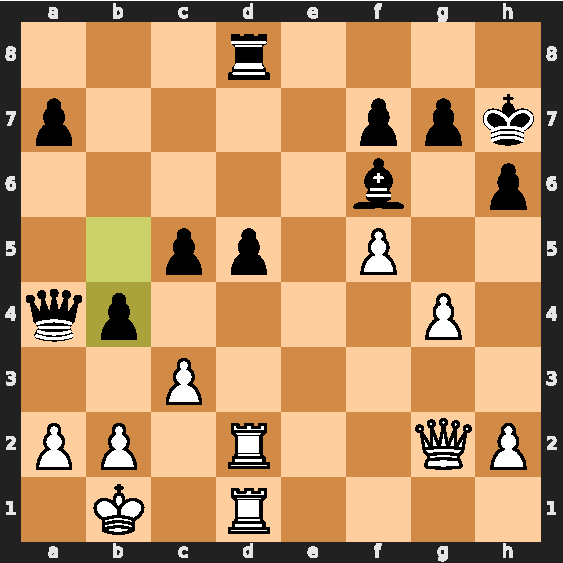
\includegraphics[width=\boardwidth]{diagrams/board-427500257a32}}}

\Move{\href{https://lichess.org/analysis/pgn/e4_e5_d4_exd4_Qxd4_Nc6_Qe3_Nf6_Nc3_Bb4_Bd2_O-O_O-O-O_Re8_Qg3_Nxe4_Nxe4_Rxe4_Bf4_Qf6_Nh3_d6_Bd3_Nd4_Be3_Bg4_Ng5_Rxe3_Qxg4_Ne2_Bxe2_Rxe2_Ne4_Rxe4_Qxe4_Qg5_f4_Qb5_c3_Bc5_Rhe1_Qc6_Rd5_Qd7_f5_c6_Rd2_d5_Qf3_Be7_Rde2_Bf6_Qh5_h6_g4_Kh7_Kb1_Rd8_Rd1_c5_Qh3_Qa4_Red2_Qe4_Ka1_b5_Qg2_Qa4_Kb1_b4_cxb4}{36.cxb4} \href{https://lichess.org/analysis/pgn/e4_e5_d4_exd4_Qxd4_Nc6_Qe3_Nf6_Nc3_Bb4_Bd2_O-O_O-O-O_Re8_Qg3_Nxe4_Nxe4_Rxe4_Bf4_Qf6_Nh3_d6_Bd3_Nd4_Be3_Bg4_Ng5_Rxe3_Qxg4_Ne2_Bxe2_Rxe2_Ne4_Rxe4_Qxe4_Qg5_f4_Qb5_c3_Bc5_Rhe1_Qc6_Rd5_Qd7_f5_c6_Rd2_d5_Qf3_Be7_Rde2_Bf6_Qh5_h6_g4_Kh7_Kb1_Rd8_Rd1_c5_Qh3_Qa4_Red2_Qe4_Ka1_b5_Qg2_Qa4_Kb1_b4_cxb4_Qxb4}{\figQ xb4}}

Black has now a passed Pawn, and his Bishop exerts great pressure. White cannot very well play now \href{https://lichess.org/analysis/pgn/e4_e5_d4_exd4_Qxd4_Nc6_Qe3_Nf6_Nc3_Bb4_Bd2_O-O_O-O-O_Re8_Qg3_Nxe4_Nxe4_Rxe4_Bf4_Qf6_Nh3_d6_Bd3_Nd4_Be3_Bg4_Ng5_Rxe3_Qxg4_Ne2_Bxe2_Rxe2_Ne4_Rxe4_Qxe4_Qg5_f4_Qb5_c3_Bc5_Rhe1_Qc6_Rd5_Qd7_f5_c6_Rd2_d5_Qf3_Be7_Rde2_Bf6_Qh5_h6_g4_Kh7_Kb1_Rd8_Rd1_c5_Qh3_Qa4_Red2_Qe4_Ka1_b5_Qg2_Qa4_Kb1_b4_cxb4_Qxb4_Rxd5}{37.\figR xd5} because of \href{https://lichess.org/analysis/pgn/e4_e5_d4_exd4_Qxd4_Nc6_Qe3_Nf6_Nc3_Bb4_Bd2_O-O_O-O-O_Re8_Qg3_Nxe4_Nxe4_Rxe4_Bf4_Qf6_Nh3_d6_Bd3_Nd4_Be3_Bg4_Ng5_Rxe3_Qxg4_Ne2_Bxe2_Rxe2_Ne4_Rxe4_Qxe4_Qg5_f4_Qb5_c3_Bc5_Rhe1_Qc6_Rd5_Qd7_f5_c6_Rd2_d5_Qf3_Be7_Rde2_Bf6_Qh5_h6_g4_Kh7_Kb1_Rd8_Rd1_c5_Qh3_Qa4_Red2_Qe4_Ka1_b5_Qg2_Qa4_Kb1_b4_cxb4_Qxb4_Rxd5_Rxd5}{37...\figR xd5} \href{https://lichess.org/analysis/pgn/e4_e5_d4_exd4_Qxd4_Nc6_Qe3_Nf6_Nc3_Bb4_Bd2_O-O_O-O-O_Re8_Qg3_Nxe4_Nxe4_Rxe4_Bf4_Qf6_Nh3_d6_Bd3_Nd4_Be3_Bg4_Ng5_Rxe3_Qxg4_Ne2_Bxe2_Rxe2_Ne4_Rxe4_Qxe4_Qg5_f4_Qb5_c3_Bc5_Rhe1_Qc6_Rd5_Qd7_f5_c6_Rd2_d5_Qf3_Be7_Rde2_Bf6_Qh5_h6_g4_Kh7_Kb1_Rd8_Rd1_c5_Qh3_Qa4_Red2_Qe4_Ka1_b5_Qg2_Qa4_Kb1_b4_cxb4_Qxb4_Rxd5_Rxd5_Rxd5}{38.\figR xd5} \href{https://lichess.org/analysis/pgn/e4_e5_d4_exd4_Qxd4_Nc6_Qe3_Nf6_Nc3_Bb4_Bd2_O-O_O-O-O_Re8_Qg3_Nxe4_Nxe4_Rxe4_Bf4_Qf6_Nh3_d6_Bd3_Nd4_Be3_Bg4_Ng5_Rxe3_Qxg4_Ne2_Bxe2_Rxe2_Ne4_Rxe4_Qxe4_Qg5_f4_Qb5_c3_Bc5_Rhe1_Qc6_Rd5_Qd7_f5_c6_Rd2_d5_Qf3_Be7_Rde2_Bf6_Qh5_h6_g4_Kh7_Kb1_Rd8_Rd1_c5_Qh3_Qa4_Red2_Qe4_Ka1_b5_Qg2_Qa4_Kb1_b4_cxb4_Qxb4_Rxd5_Rxd5_Rxd5_Bxb2}{\figB xb2}; and White could not take the Bishop because \figQ e4+ would win the Rook, leaving Black a clear passed Pawn ahead.

\Move{\href{https://lichess.org/analysis/pgn/e4_e5_d4_exd4_Qxd4_Nc6_Qe3_Nf6_Nc3_Bb4_Bd2_O-O_O-O-O_Re8_Qg3_Nxe4_Nxe4_Rxe4_Bf4_Qf6_Nh3_d6_Bd3_Nd4_Be3_Bg4_Ng5_Rxe3_Qxg4_Ne2_Bxe2_Rxe2_Ne4_Rxe4_Qxe4_Qg5_f4_Qb5_c3_Bc5_Rhe1_Qc6_Rd5_Qd7_f5_c6_Rd2_d5_Qf3_Be7_Rde2_Bf6_Qh5_h6_g4_Kh7_Kb1_Rd8_Rd1_c5_Qh3_Qa4_Red2_Qe4_Ka1_b5_Qg2_Qa4_Kb1_b4_cxb4_Qxb4_a3}{37.a3} \href{https://lichess.org/analysis/pgn/e4_e5_d4_exd4_Qxd4_Nc6_Qe3_Nf6_Nc3_Bb4_Bd2_O-O_O-O-O_Re8_Qg3_Nxe4_Nxe4_Rxe4_Bf4_Qf6_Nh3_d6_Bd3_Nd4_Be3_Bg4_Ng5_Rxe3_Qxg4_Ne2_Bxe2_Rxe2_Ne4_Rxe4_Qxe4_Qg5_f4_Qb5_c3_Bc5_Rhe1_Qc6_Rd5_Qd7_f5_c6_Rd2_d5_Qf3_Be7_Rde2_Bf6_Qh5_h6_g4_Kh7_Kb1_Rd8_Rd1_c5_Qh3_Qa4_Red2_Qe4_Ka1_b5_Qg2_Qa4_Kb1_b4_cxb4_Qxb4_a3_Qa4}{\figQ a4!} \href{https://lichess.org/analysis/pgn/e4_e5_d4_exd4_Qxd4_Nc6_Qe3_Nf6_Nc3_Bb4_Bd2_O-O_O-O-O_Re8_Qg3_Nxe4_Nxe4_Rxe4_Bf4_Qf6_Nh3_d6_Bd3_Nd4_Be3_Bg4_Ng5_Rxe3_Qxg4_Ne2_Bxe2_Rxe2_Ne4_Rxe4_Qxe4_Qg5_f4_Qb5_c3_Bc5_Rhe1_Qc6_Rd5_Qd7_f5_c6_Rd2_d5_Qf3_Be7_Rde2_Bf6_Qh5_h6_g4_Kh7_Kb1_Rd8_Rd1_c5_Qh3_Qa4_Red2_Qe4_Ka1_b5_Qg2_Qa4_Kb1_b4_cxb4_Qxb4_a3_Qa4_Rxd5}{38.\figR xd5} \href{https://lichess.org/analysis/pgn/e4_e5_d4_exd4_Qxd4_Nc6_Qe3_Nf6_Nc3_Bb4_Bd2_O-O_O-O-O_Re8_Qg3_Nxe4_Nxe4_Rxe4_Bf4_Qf6_Nh3_d6_Bd3_Nd4_Be3_Bg4_Ng5_Rxe3_Qxg4_Ne2_Bxe2_Rxe2_Ne4_Rxe4_Qxe4_Qg5_f4_Qb5_c3_Bc5_Rhe1_Qc6_Rd5_Qd7_f5_c6_Rd2_d5_Qf3_Be7_Rde2_Bf6_Qh5_h6_g4_Kh7_Kb1_Rd8_Rd1_c5_Qh3_Qa4_Red2_Qe4_Ka1_b5_Qg2_Qa4_Kb1_b4_cxb4_Qxb4_a3_Qa4_Rxd5_Rb8}{\figR b8} \href{https://lichess.org/analysis/pgn/e4_e5_d4_exd4_Qxd4_Nc6_Qe3_Nf6_Nc3_Bb4_Bd2_O-O_O-O-O_Re8_Qg3_Nxe4_Nxe4_Rxe4_Bf4_Qf6_Nh3_d6_Bd3_Nd4_Be3_Bg4_Ng5_Rxe3_Qxg4_Ne2_Bxe2_Rxe2_Ne4_Rxe4_Qxe4_Qg5_f4_Qb5_c3_Bc5_Rhe1_Qc6_Rd5_Qd7_f5_c6_Rd2_d5_Qf3_Be7_Rde2_Bf6_Qh5_h6_g4_Kh7_Kb1_Rd8_Rd1_c5_Qh3_Qa4_Red2_Qe4_Ka1_b5_Qg2_Qa4_Kb1_b4_cxb4_Qxb4_a3_Qa4_Rxd5_Rb8_R1d2}{39.\figR 1d2} \href{https://lichess.org/analysis/pgn/e4_e5_d4_exd4_Qxd4_Nc6_Qe3_Nf6_Nc3_Bb4_Bd2_O-O_O-O-O_Re8_Qg3_Nxe4_Nxe4_Rxe4_Bf4_Qf6_Nh3_d6_Bd3_Nd4_Be3_Bg4_Ng5_Rxe3_Qxg4_Ne2_Bxe2_Rxe2_Ne4_Rxe4_Qxe4_Qg5_f4_Qb5_c3_Bc5_Rhe1_Qc6_Rd5_Qd7_f5_c6_Rd2_d5_Qf3_Be7_Rde2_Bf6_Qh5_h6_g4_Kh7_Kb1_Rd8_Rd1_c5_Qh3_Qa4_Red2_Qe4_Ka1_b5_Qg2_Qa4_Kb1_b4_cxb4_Qxb4_a3_Qa4_Rxd5_Rb8_R1d2_c4}{c4} \href{https://lichess.org/analysis/pgn/e4_e5_d4_exd4_Qxd4_Nc6_Qe3_Nf6_Nc3_Bb4_Bd2_O-O_O-O-O_Re8_Qg3_Nxe4_Nxe4_Rxe4_Bf4_Qf6_Nh3_d6_Bd3_Nd4_Be3_Bg4_Ng5_Rxe3_Qxg4_Ne2_Bxe2_Rxe2_Ne4_Rxe4_Qxe4_Qg5_f4_Qb5_c3_Bc5_Rhe1_Qc6_Rd5_Qd7_f5_c6_Rd2_d5_Qf3_Be7_Rde2_Bf6_Qh5_h6_g4_Kh7_Kb1_Rd8_Rd1_c5_Qh3_Qa4_Red2_Qe4_Ka1_b5_Qg2_Qa4_Kb1_b4_cxb4_Qxb4_a3_Qa4_Rxd5_Rb8_R1d2_c4_Qg3}{40.\figQ g3} \href{https://lichess.org/analysis/pgn/e4_e5_d4_exd4_Qxd4_Nc6_Qe3_Nf6_Nc3_Bb4_Bd2_O-O_O-O-O_Re8_Qg3_Nxe4_Nxe4_Rxe4_Bf4_Qf6_Nh3_d6_Bd3_Nd4_Be3_Bg4_Ng5_Rxe3_Qxg4_Ne2_Bxe2_Rxe2_Ne4_Rxe4_Qxe4_Qg5_f4_Qb5_c3_Bc5_Rhe1_Qc6_Rd5_Qd7_f5_c6_Rd2_d5_Qf3_Be7_Rde2_Bf6_Qh5_h6_g4_Kh7_Kb1_Rd8_Rd1_c5_Qh3_Qa4_Red2_Qe4_Ka1_b5_Qg2_Qa4_Kb1_b4_cxb4_Qxb4_a3_Qa4_Rxd5_Rb8_R1d2_c4_Qg3_Rb3}{\figR b3} \href{https://lichess.org/analysis/pgn/e4_e5_d4_exd4_Qxd4_Nc6_Qe3_Nf6_Nc3_Bb4_Bd2_O-O_O-O-O_Re8_Qg3_Nxe4_Nxe4_Rxe4_Bf4_Qf6_Nh3_d6_Bd3_Nd4_Be3_Bg4_Ng5_Rxe3_Qxg4_Ne2_Bxe2_Rxe2_Ne4_Rxe4_Qxe4_Qg5_f4_Qb5_c3_Bc5_Rhe1_Qc6_Rd5_Qd7_f5_c6_Rd2_d5_Qf3_Be7_Rde2_Bf6_Qh5_h6_g4_Kh7_Kb1_Rd8_Rd1_c5_Qh3_Qa4_Red2_Qe4_Ka1_b5_Qg2_Qa4_Kb1_b4_cxb4_Qxb4_a3_Qa4_Rxd5_Rb8_R1d2_c4_Qg3_Rb3_Qd6}{41.\figQ d6}}

\ChessDiagram{\href{https://lichess.org/analysis/pgn/e4_e5_d4_exd4_Qxd4_Nc6_Qe3_Nf6_Nc3_Bb4_Bd2_O-O_O-O-O_Re8_Qg3_Nxe4_Nxe4_Rxe4_Bf4_Qf6_Nh3_d6_Bd3_Nd4_Be3_Bg4_Ng5_Rxe3_Qxg4_Ne2_Bxe2_Rxe2_Ne4_Rxe4_Qxe4_Qg5_f4_Qb5_c3_Bc5_Rhe1_Qc6_Rd5_Qd7_f5_c6_Rd2_d5_Qf3_Be7_Rde2_Bf6_Qh5_h6_g4_Kh7_Kb1_Rd8_Rd1_c5_Qh3_Qa4_Red2_Qe4_Ka1_b5_Qg2_Qa4_Kb1_b4_cxb4_Qxb4_a3_Qa4_Rxd5_Rb8_R1d2_c4_Qg3_Rb3_Qd6}{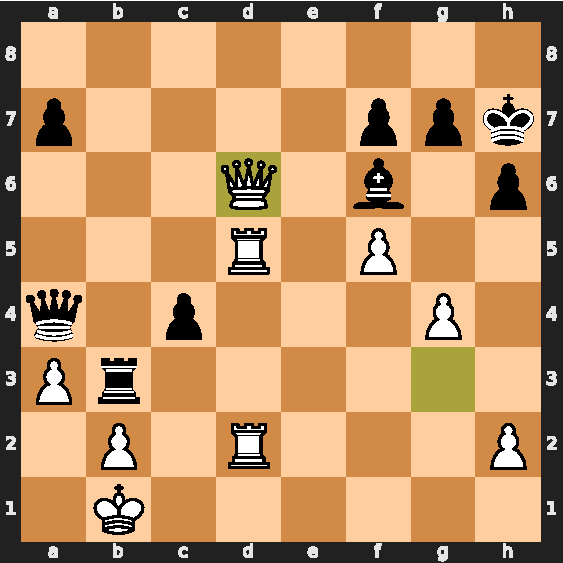
\includegraphics[width=\boardwidth]{diagrams/board-b44a0081f321}}}

\Move{\href{https://lichess.org/analysis/pgn/e4_e5_d4_exd4_Qxd4_Nc6_Qe3_Nf6_Nc3_Bb4_Bd2_O-O_O-O-O_Re8_Qg3_Nxe4_Nxe4_Rxe4_Bf4_Qf6_Nh3_d6_Bd3_Nd4_Be3_Bg4_Ng5_Rxe3_Qxg4_Ne2_Bxe2_Rxe2_Ne4_Rxe4_Qxe4_Qg5_f4_Qb5_c3_Bc5_Rhe1_Qc6_Rd5_Qd7_f5_c6_Rd2_d5_Qf3_Be7_Rde2_Bf6_Qh5_h6_g4_Kh7_Kb1_Rd8_Rd1_c5_Qh3_Qa4_Red2_Qe4_Ka1_b5_Qg2_Qa4_Kb1_b4_cxb4_Qxb4_a3_Qa4_Rxd5_Rb8_R1d2_c4_Qg3_Rb3_Qd6_c3}{41...c3}}

\href{https://lichess.org/analysis/pgn/e4_e5_d4_exd4_Qxd4_Nc6_Qe3_Nf6_Nc3_Bb4_Bd2_O-O_O-O-O_Re8_Qg3_Nxe4_Nxe4_Rxe4_Bf4_Qf6_Nh3_d6_Bd3_Nd4_Be3_Bg4_Ng5_Rxe3_Qxg4_Ne2_Bxe2_Rxe2_Ne4_Rxe4_Qxe4_Qg5_f4_Qb5_c3_Bc5_Rhe1_Qc6_Rd5_Qd7_f5_c6_Rd2_d5_Qf3_Be7_Rde2_Bf6_Qh5_h6_g4_Kh7_Kb1_Rd8_Rd1_c5_Qh3_Qa4_Red2_Qe4_Ka1_b5_Qg2_Qa4_Kb1_b4_cxb4_Qxb4_a3_Qa4_Rxd5_Rb8_R1d2_c4_Qg3_Rb3_Qd6_Bxb2}{41...\figB xb2} would also win, which shows that White's game is altogether gone. In these cases, however, it is not the prettiest move that should be played, but the most effective one, the move that will make your opponent resign soonest.

\Move{\href{https://lichess.org/analysis/pgn/e4_e5_d4_exd4_Qxd4_Nc6_Qe3_Nf6_Nc3_Bb4_Bd2_O-O_O-O-O_Re8_Qg3_Nxe4_Nxe4_Rxe4_Bf4_Qf6_Nh3_d6_Bd3_Nd4_Be3_Bg4_Ng5_Rxe3_Qxg4_Ne2_Bxe2_Rxe2_Ne4_Rxe4_Qxe4_Qg5_f4_Qb5_c3_Bc5_Rhe1_Qc6_Rd5_Qd7_f5_c6_Rd2_d5_Qf3_Be7_Rde2_Bf6_Qh5_h6_g4_Kh7_Kb1_Rd8_Rd1_c5_Qh3_Qa4_Red2_Qe4_Ka1_b5_Qg2_Qa4_Kb1_b4_cxb4_Qxb4_a3_Qa4_Rxd5_Rb8_R1d2_c4_Qg3_Rb3_Qd6_c3_Rc2}{42.\figR c2} \href{https://lichess.org/analysis/pgn/e4_e5_d4_exd4_Qxd4_Nc6_Qe3_Nf6_Nc3_Bb4_Bd2_O-O_O-O-O_Re8_Qg3_Nxe4_Nxe4_Rxe4_Bf4_Qf6_Nh3_d6_Bd3_Nd4_Be3_Bg4_Ng5_Rxe3_Qxg4_Ne2_Bxe2_Rxe2_Ne4_Rxe4_Qxe4_Qg5_f4_Qb5_c3_Bc5_Rhe1_Qc6_Rd5_Qd7_f5_c6_Rd2_d5_Qf3_Be7_Rde2_Bf6_Qh5_h6_g4_Kh7_Kb1_Rd8_Rd1_c5_Qh3_Qa4_Red2_Qe4_Ka1_b5_Qg2_Qa4_Kb1_b4_cxb4_Qxb4_a3_Qa4_Rxd5_Rb8_R1d2_c4_Qg3_Rb3_Qd6_c3_Rc2_cxb2}{cxb2} \href{https://lichess.org/analysis/pgn/e4_e5_d4_exd4_Qxd4_Nc6_Qe3_Nf6_Nc3_Bb4_Bd2_O-O_O-O-O_Re8_Qg3_Nxe4_Nxe4_Rxe4_Bf4_Qf6_Nh3_d6_Bd3_Nd4_Be3_Bg4_Ng5_Rxe3_Qxg4_Ne2_Bxe2_Rxe2_Ne4_Rxe4_Qxe4_Qg5_f4_Qb5_c3_Bc5_Rhe1_Qc6_Rd5_Qd7_f5_c6_Rd2_d5_Qf3_Be7_Rde2_Bf6_Qh5_h6_g4_Kh7_Kb1_Rd8_Rd1_c5_Qh3_Qa4_Red2_Qe4_Ka1_b5_Qg2_Qa4_Kb1_b4_cxb4_Qxb4_a3_Qa4_Rxd5_Rb8_R1d2_c4_Qg3_Rb3_Qd6_c3_Rc2_cxb2_Rd3}{43.\figR d3} \href{https://lichess.org/analysis/pgn/e4_e5_d4_exd4_Qxd4_Nc6_Qe3_Nf6_Nc3_Bb4_Bd2_O-O_O-O-O_Re8_Qg3_Nxe4_Nxe4_Rxe4_Bf4_Qf6_Nh3_d6_Bd3_Nd4_Be3_Bg4_Ng5_Rxe3_Qxg4_Ne2_Bxe2_Rxe2_Ne4_Rxe4_Qxe4_Qg5_f4_Qb5_c3_Bc5_Rhe1_Qc6_Rd5_Qd7_f5_c6_Rd2_d5_Qf3_Be7_Rde2_Bf6_Qh5_h6_g4_Kh7_Kb1_Rd8_Rd1_c5_Qh3_Qa4_Red2_Qe4_Ka1_b5_Qg2_Qa4_Kb1_b4_cxb4_Qxb4_a3_Qa4_Rxd5_Rb8_R1d2_c4_Qg3_Rb3_Qd6_c3_Rc2_cxb2_Rd3_Qe4}{\figQ e4!} \href{https://lichess.org/analysis/pgn/e4_e5_d4_exd4_Qxd4_Nc6_Qe3_Nf6_Nc3_Bb4_Bd2_O-O_O-O-O_Re8_Qg3_Nxe4_Nxe4_Rxe4_Bf4_Qf6_Nh3_d6_Bd3_Nd4_Be3_Bg4_Ng5_Rxe3_Qxg4_Ne2_Bxe2_Rxe2_Ne4_Rxe4_Qxe4_Qg5_f4_Qb5_c3_Bc5_Rhe1_Qc6_Rd5_Qd7_f5_c6_Rd2_d5_Qf3_Be7_Rde2_Bf6_Qh5_h6_g4_Kh7_Kb1_Rd8_Rd1_c5_Qh3_Qa4_Red2_Qe4_Ka1_b5_Qg2_Qa4_Kb1_b4_cxb4_Qxb4_a3_Qa4_Rxd5_Rb8_R1d2_c4_Qg3_Rb3_Qd6_c3_Rc2_cxb2_Rd3_Qe4_Rd1}{44.\figR d1} \href{https://lichess.org/analysis/pgn/e4_e5_d4_exd4_Qxd4_Nc6_Qe3_Nf6_Nc3_Bb4_Bd2_O-O_O-O-O_Re8_Qg3_Nxe4_Nxe4_Rxe4_Bf4_Qf6_Nh3_d6_Bd3_Nd4_Be3_Bg4_Ng5_Rxe3_Qxg4_Ne2_Bxe2_Rxe2_Ne4_Rxe4_Qxe4_Qg5_f4_Qb5_c3_Bc5_Rhe1_Qc6_Rd5_Qd7_f5_c6_Rd2_d5_Qf3_Be7_Rde2_Bf6_Qh5_h6_g4_Kh7_Kb1_Rd8_Rd1_c5_Qh3_Qa4_Red2_Qe4_Ka1_b5_Qg2_Qa4_Kb1_b4_cxb4_Qxb4_a3_Qa4_Rxd5_Rb8_R1d2_c4_Qg3_Rb3_Qd6_c3_Rc2_cxb2_Rd3_Qe4_Rd1_Rc3}{\figR c3}}

\noindent\textbf{Resigns.}

Of course White must play \href{https://lichess.org/analysis/pgn/e4_e5_d4_exd4_Qxd4_Nc6_Qe3_Nf6_Nc3_Bb4_Bd2_O-O_O-O-O_Re8_Qg3_Nxe4_Nxe4_Rxe4_Bf4_Qf6_Nh3_d6_Bd3_Nd4_Be3_Bg4_Ng5_Rxe3_Qxg4_Ne2_Bxe2_Rxe2_Ne4_Rxe4_Qxe4_Qg5_f4_Qb5_c3_Bc5_Rhe1_Qc6_Rd5_Qd7_f5_c6_Rd2_d5_Qf3_Be7_Rde2_Bf6_Qh5_h6_g4_Kh7_Kb1_Rd8_Rd1_c5_Qh3_Qa4_Red2_Qe4_Ka1_b5_Qg2_Qa4_Kb1_b4_cxb4_Qxb4_a3_Qa4_Rxd5_Rb8_R1d2_c4_Qg3_Rb3_Qd6_c3_Rc2_cxb2_Rd3_Qe4_Rd1_Rc3_Qd2}{45.\figQ d2}, and Black then plays \href{https://lichess.org/analysis/pgn/e4_e5_d4_exd4_Qxd4_Nc6_Qe3_Nf6_Nc3_Bb4_Bd2_O-O_O-O-O_Re8_Qg3_Nxe4_Nxe4_Rxe4_Bf4_Qf6_Nh3_d6_Bd3_Nd4_Be3_Bg4_Ng5_Rxe3_Qxg4_Ne2_Bxe2_Rxe2_Ne4_Rxe4_Qxe4_Qg5_f4_Qb5_c3_Bc5_Rhe1_Qc6_Rd5_Qd7_f5_c6_Rd2_d5_Qf3_Be7_Rde2_Bf6_Qh5_h6_g4_Kh7_Kb1_Rd8_Rd1_c5_Qh3_Qa4_Red2_Qe4_Ka1_b5_Qg2_Qa4_Kb1_b4_cxb4_Qxb4_a3_Qa4_Rxd5_Rb8_R1d2_c4_Qg3_Rb3_Qd6_c3_Rc2_cxb2_Rd3_Qe4_Rd1_Rc3_Qd2_Rxa3}{45...\figR xa3}.

\end{document}
